% !TEX root = ../thesis.tex
Adiabatic capture theory is a study of the long range potentials between particles to yield a reaction rate constant. This is easily done for many potentials, such as the ion and induced-dipole interaction (Langevin), but is more difficult when considering potentials with another degree of freedom; in particular, we would like to consider the ion-dipole interaction. Unlike the Langevin interaction, the ion-dipole term has an angular term defined with respect to the inter-molecular axis. A few approximations are taken to give an average dipole orientation theory pioneered and expanded on by Su and Bowers.\cite{Su1973, Su1973a} This can also be extrapolated to include quadrupole interactions.\cite{Su1975}

\subsection{General Treatment of Adiabatic Capture Theory} \label{sec: ACT}
A general method of calculating the rate constant of two particles with a given potential, finding the collisional cross section, which is then averaged over a velocity distribution to find the rate constant.\cite{Zhang2017} Starting with the attractive potential, we find that it is a summation of interactions with coefficients $C_n$ and $r$ dependence $n$.

\begin{equation}
    V(r) = \sum_n -\frac{C_n}{r^n}
\end{equation}

In the center of mass frame, we see that

\begin{equation}
    V_{eff} = \frac{l^2}{2 \mu r^2} - \sum_n \frac{C_n}{r^n}\label{eq: veff}
\end{equation}

if $n > 2$, we can derive the capture cross-section and rate constant as follows. First, we find the position $r_0$ corresponding to the maximum of the effective potential, which is the maximum of the centrifugal barrier.

\begin{align*}
    \frac{\partial V_{eff}(r_0)}{\partial r} & = 0 \\
    \therefore r_0 & = \left(\frac{n \mu, C_n}{l^2}\right)^{1/n-2}
\end{align*}

Substituting $r_0$ back into equation $\ref{eq: veff}$, we find the maximal value of the effective potential:

\begin{equation}
    V_{eff}(r_0) = \left(\frac{l^2}{\mu}\right)^{\frac{n}{n-2}} \frac{n-2}{2n}(n C_n)^{-\frac{2}{n-2}}
\end{equation}

This then defines the energy necessary for a collision, for if $E_{col}$ exceeds $V_{eff}(r_0)$, the reactants will be able to surmount the centrifugal barrier and collide. Thus, we may define the maximum value for the angular momentum $l$ and the impact parameter $b$.

\begin{align*}
    l_{max} & = (\mu n)^{1/2}(C_n)^{1/n} \left(\frac{2 E_{col}}{n-2}\right)^{\frac{n-2}{2n}} \\
    b_{max} & = \frac{l_{max}}{\mu v}
\end{align*}

We can then define a collision cross section dependent on the collision energy:

\begin{align*}
    \sigma(E_{col}) & = \pi b^2_{max} \\
    & = \frac{\pi}{2} n \left(\frac{2}{n-2}\right)^{\frac{n-2}{2}} \left(\frac{C_n}{E_{col}}\right)^{\frac{2}{n}}
\end{align*}

Integrating the collision cross section with a Maxwell Boltzmann distribution yields a generalized rate constant as a function of temperature and n.

\begin{align}
    k(T) & = \int_0^{\infty} v f(v) \sigma(v) dv \label{eq: k int} \\
    & = \boxed{\sqrt{\frac{2 \pi}{\mu}}n\left(\frac{2}{n-2}\right)^{\frac{n-2}{2}}C_n^{2/n}(k_B T)^{\frac{n-4}{2n}}\Gamma\left(2-\frac{2}{n}\right)} \label{eq: k(T)}
\end{align}

\subsection{Ion-Dipole Interaction}

The Langevin term of the ion and ion-induced dipole interaction is as follows:

\begin{align}
V_L(r)= &-\frac{\alpha q^2}{2r^4}
\end{align}

In the case of the ion-dipole interaction:

\begin{align}
V_D(r, \theta) = & -\frac{q\mu_D}{r^2} \cos(\theta)
\end{align}

The method outlined in section \ref{sec: ACT} finds the rate constant by dealing with a two body problem only needing to consider the $r$ degree of freedom. The inclusion of the $\theta$ term complicates this, but to first order, we can parameterize it as a function of $r$. What we want to achieve is to write down the potential as such:

\begin{align}
    V(r) & = -\frac{\alpha q^2}{2r^4} - \frac{q\mu_D}{r^2} \cos\left(\bar{\theta}(r)\right) \nonumber \\
    \bar{\theta} & = \frac{\int \theta P(\theta) d\theta}{\int P(\theta) d\theta} \label{eq: avg theta}
\end{align}

Where $P(\theta)$ is the probability of finding the dipole at $\theta$. To determine the average orientation of the dipole, we consider the following cases:

\begin{enumerate}
	\item $P(\theta)$ is inversely proportional to the angular velocity:
	$$P(\theta) \propto 1/\dot{\theta}$$
	\item An orientation has a probability weighted by the circumference of an angle:
	$$C=2\pi l \sin(\theta)$$
	$$ P(\theta) \propto \sin(\theta) $$
\end{enumerate}

The angular probability is proportional to both effects:

\begin{align}
    P(\theta) & \propto \frac{\sin(\theta)}{\dot{\theta}} \label{eq: prob}
\end{align}

We can relate the angular velocity to the angular kinetic energy and the total energy in the system:
\begin{align}
    KE_{rot} & = \frac{1}{2}I\dot{\theta}^2 \nonumber \\
    E_{tot} & = KE_{rot} + V_D \label{eq: Etot}
\end{align}

Redefining equation \ref{eq: prob} with equation \ref{eq: Etot}, we find:
\begin{align}
    P(\theta) \propto & \frac{\sin(\theta)}{\sqrt{E_{rot}-V_D}} \label{eq: p theta}
\end{align}

Combining equations \cref{eq: p theta,eq: avg theta} yields a total averaged dipole orientation.

\begin{align}
    \bar{\theta} = & \frac{\int\frac{\theta \sin(\theta)d\theta}{\sqrt{E_{rot}+q\mu_D/r^2 \cos(\theta)}}}{\int\frac{\sin(\theta)d\theta}{\sqrt{E_{rot}+q\mu_D/r^2 \cos(\theta)}}} \label{eq: avg theta int}
\end{align}

From here, two situations arise:

\begin{enumerate}
	\item $E_{rot} = E_1 < \frac{q \mu_D}{r^2}$:
	There is not enough rotational energy to overcome the dipole locking. The solution is oscillatory, but $\theta$ has an $r$ dependent bound. We let the maximal capture angle be defined as $K$.

	$$ E_1=-\frac{q \mu_D}{r^2}\cos(K) $$

	When substituted into equation \ref{eq: avg theta int}, we find:

	\begin{align*}
	    \bar{\theta}_1 & = \frac{\int_0^K \frac{\theta \sin(\theta) d \theta}{\sqrt{\cos(\theta) - \cos(K)}}}{\int_0^K \frac{\sin(\theta) d \theta}{\sqrt{\cos(\theta) - \cos(K)}}}
	\end{align*}


	After some math (something something integration by infinite series) and get a result of:

	\begin{align*}
	    \bar{\theta}_1 & = \frac{2 \sqrt{2}A}{\sqrt{1-\cos(K)}} \\
	    \text{where }A & \equiv \int_0^{\pi/2} \frac{a^2 \cos(\phi)^2 d\phi}{\sqrt{q-a^2 \sin(\phi)^2}}
	\end{align*}

	\begin{figure}[H]
		\label{fig: theta1}
		\centering
		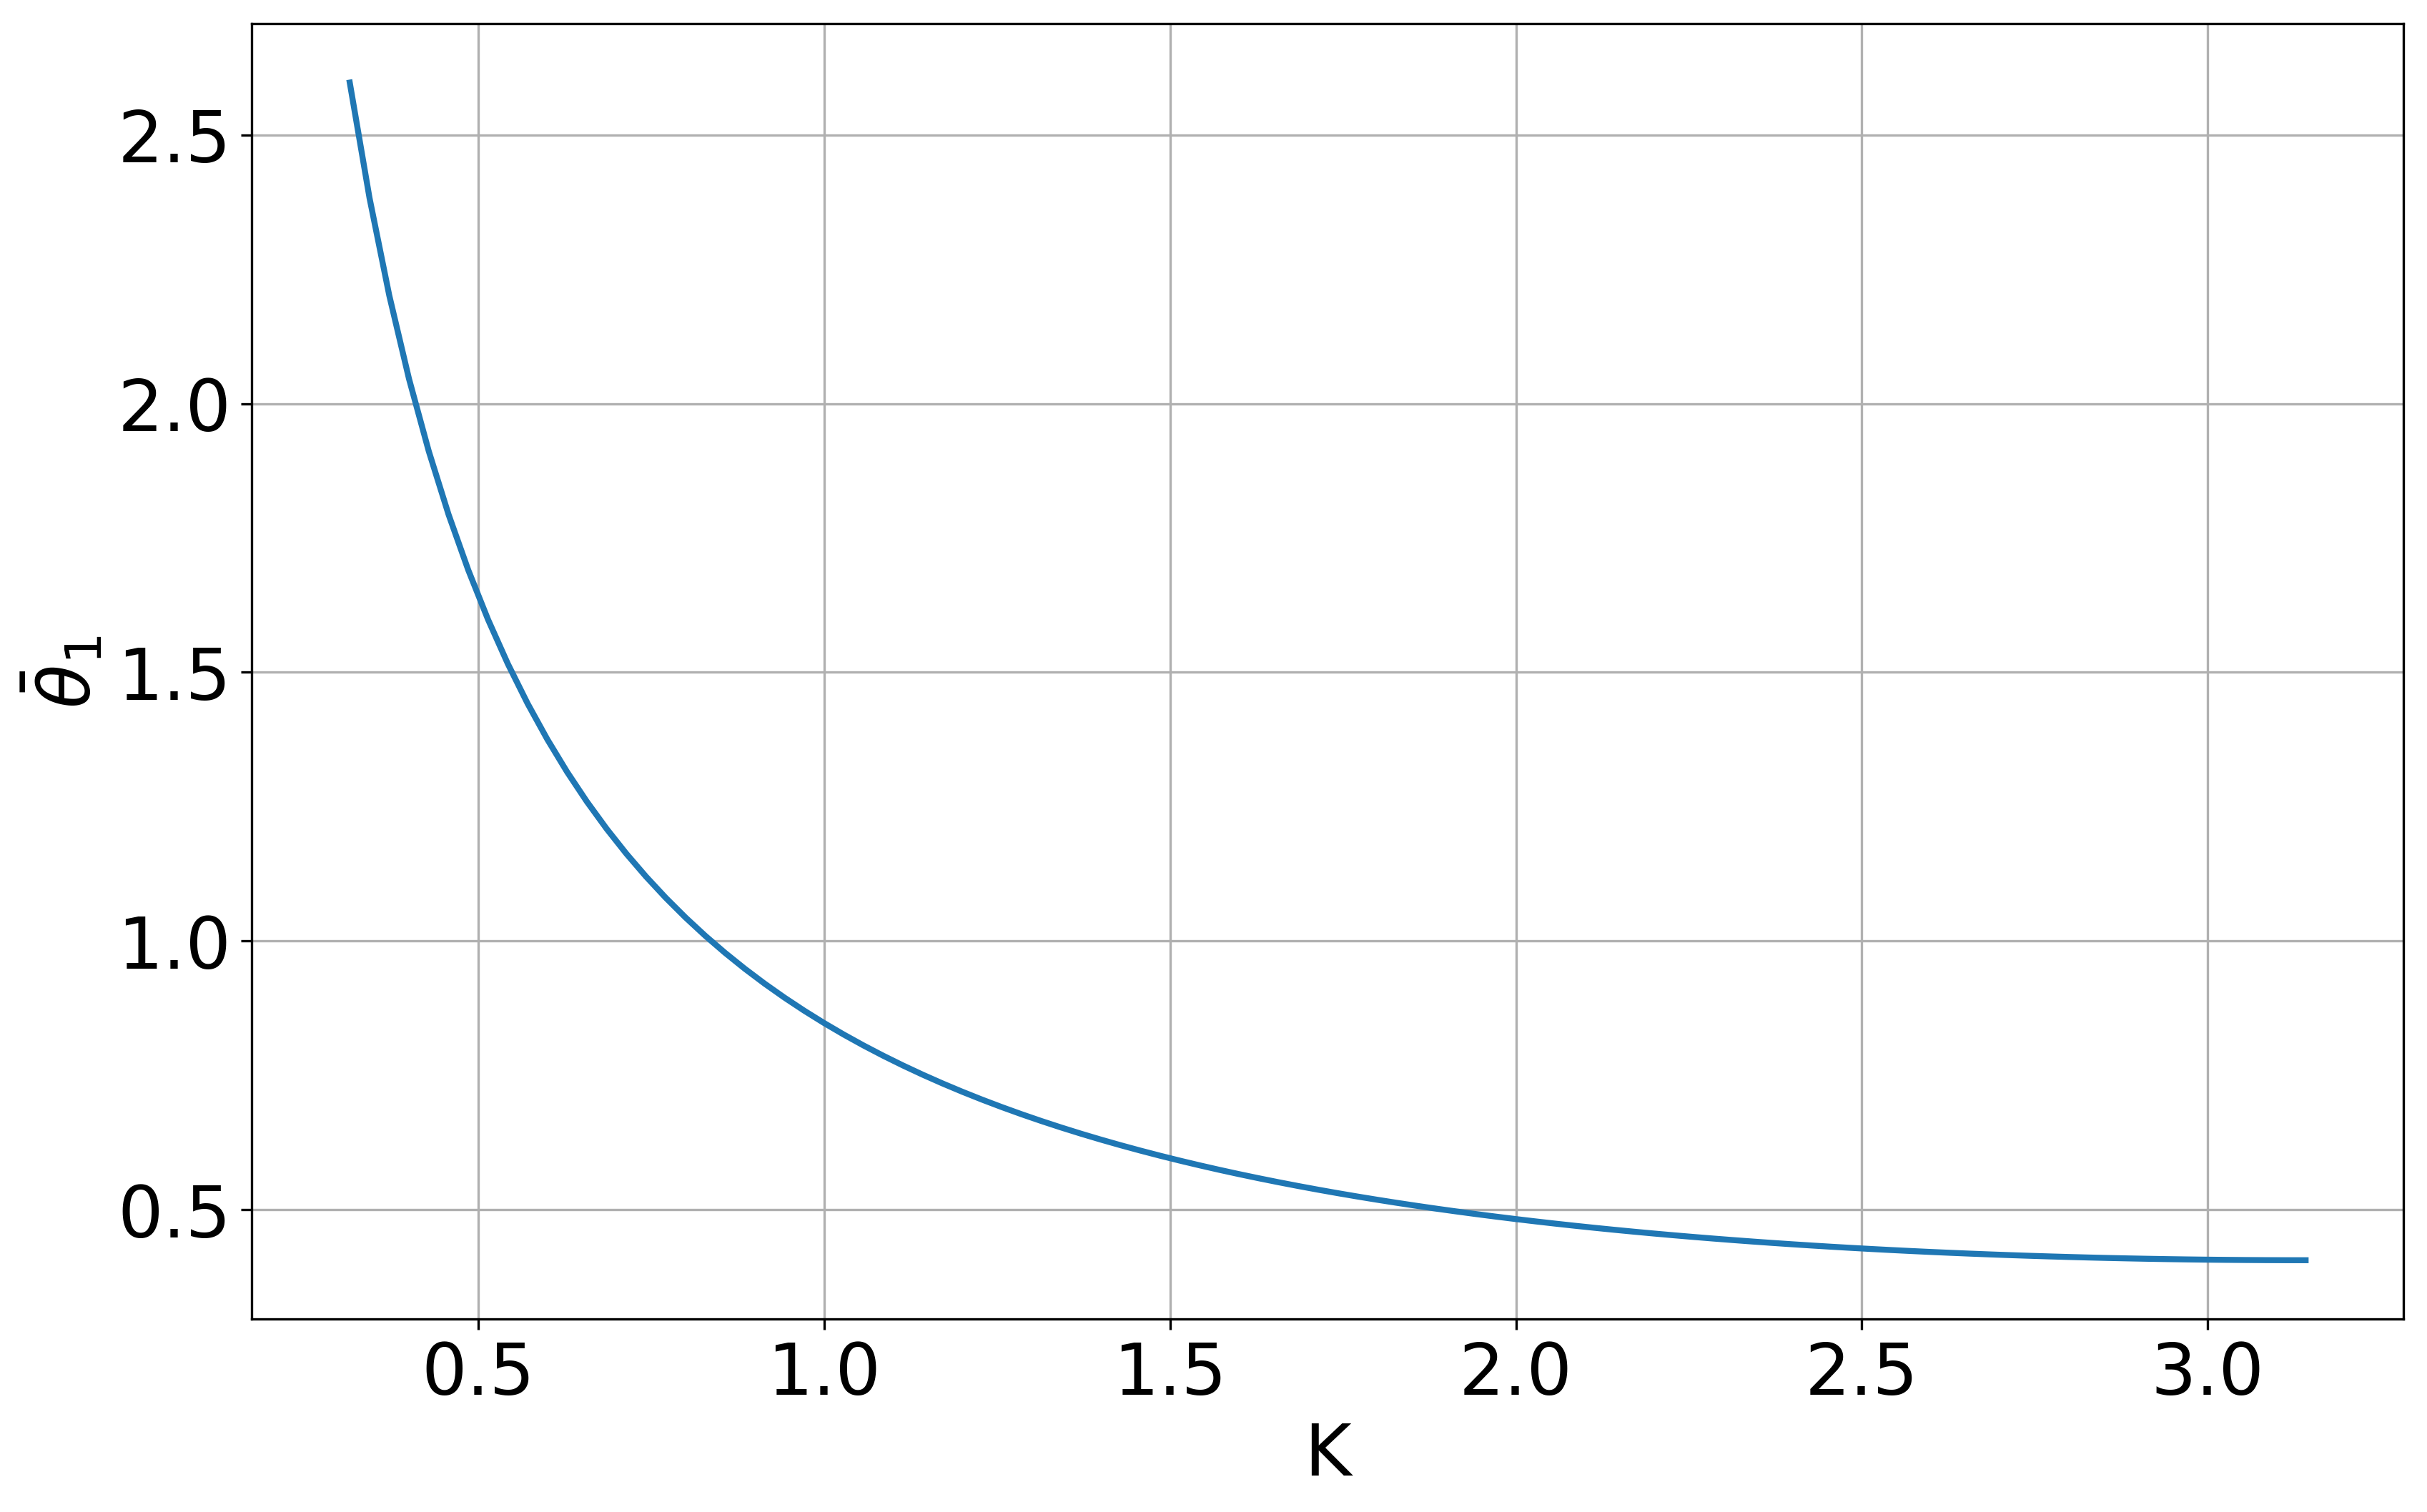
\includegraphics[width=0.8\textwidth]{images/ADO_theta1.png}
		\caption{Rough plotting of $\theta_1$ as a function of maximum angle $K$. The behaviour is as expected, the greater the maximal capture angle, the more $\theta_1$ tends towards 0.}
	\end{figure}

	\item $E_{rot} = E_1 > \frac{q \mu_D}{r^2}$:
	The rotational energy is enough to overcome the dipole locking and $\theta$ can swing around in a complete circle

	\begin{equation}
	    \bar{\theta}_2  = \frac{\int_0^\pi \frac{\theta \sin(\theta) d\theta}{\sqrt{E_2 + q \mu_D/r^2 \cos(\theta)}}}{\int_0^\pi \frac{\sin(\theta) d \theta}{\sqrt{E_2 + q \mu_D/r^2 \cos(\theta)}}}
	\end{equation}

	We no longer have bounds on the angles the dipole is allowed over, but the behaviour is still dependent on the strength of the internal energy and dipole force.

	\begin{figure}[H]
		\label{fig: theta2}
		\centering
		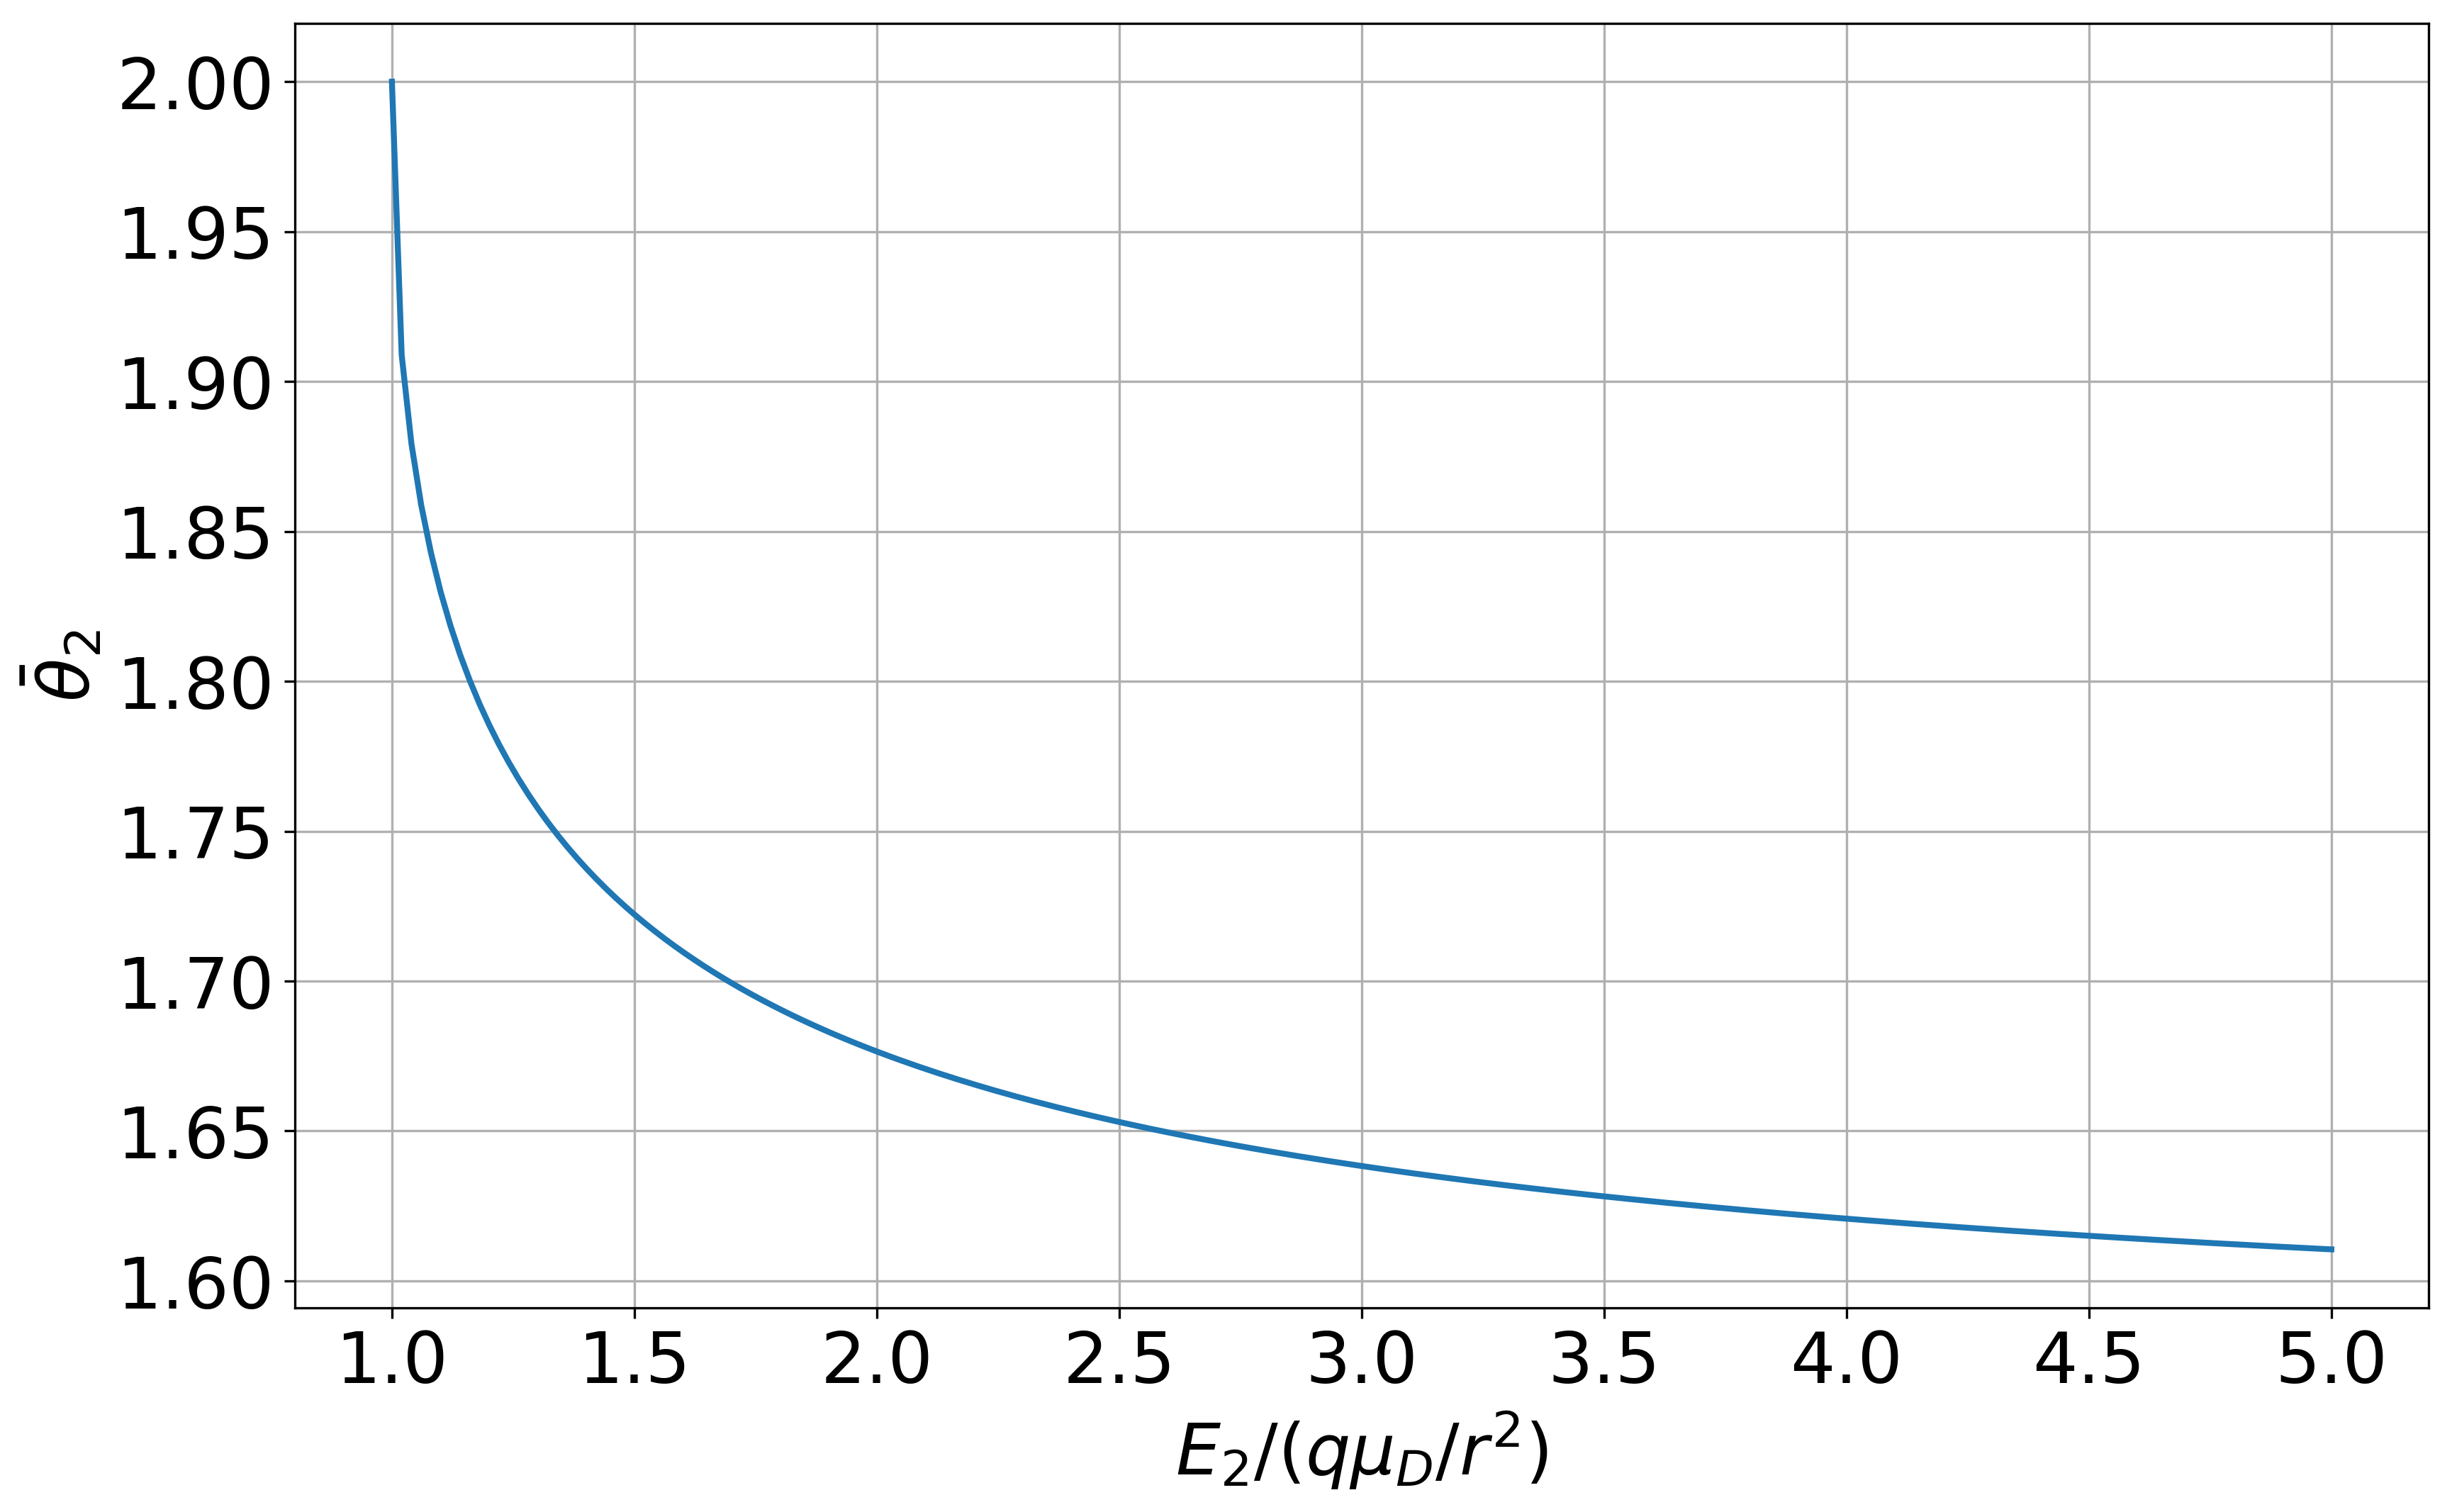
\includegraphics[width=0.8\textwidth]{images/ADO_theta2.png}
		\caption{$\theta_2$ as a function of the ratio of rotational energy and the monopole-dipole term. The low ratio behavior is not immediately obvious, but the greater the ratio between the rotational energy and monopole-dipole term, the more $\theta_2$ tends towards $\pi/2$.}
	\end{figure}

\end{enumerate}

Let's say we have the forms for $\bar{\theta_1}$ and $\bar{\theta_2}$, we want to write down the full form of $\theta$. We can combine the two weighted by the probability of each as a function of internal energy.
\begin{equation*}
    \bar{\theta}(r) = \bar{\theta}_1(r) F_1 + \bar{\theta}_2(r) F_2
\end{equation*}

Where these weightings are found via:

\begin{equation*}
    P(\epsilon) d\epsilon = \frac{1}{k_BT}e^{-\frac{\epsilon}{k_BT}}d\epsilon
\end{equation*}

For diatomics, we can use:
\begin{equation*}
    \epsilon = \frac{J(J+1)\hbar^2}{2I}
\end{equation*}

We can then use equation $\ref{eq: k int}$ and get a cross section and rate constant. The form is similar to that of just a Langevin term, but now with a dipole interaction term added onto it. All of the terms aside from $C$ come from the integration over a Boltzmann distribution, where then averaging over the angles is wrapped up into the $C$ term.

\begin{equation}
    \boxed{k_{ADO} = \frac{2 \pi e}{\sqrt{\mu}}\left(\sqrt{\alpha}+C \mu_D\sqrt{\frac{2}{\pi k_B T}}\right)}
\end{equation}

The dipole locking constant ($C$) can be numerically solved by iteratively integrating over combinations of $\mu_D$ and $\alpha$, or by looking at figure \ref{fig: C}.\cite{Su1973}\cite{Troe1985}

\begin{figure}[H]
	\label{fig: C}
	\centering
	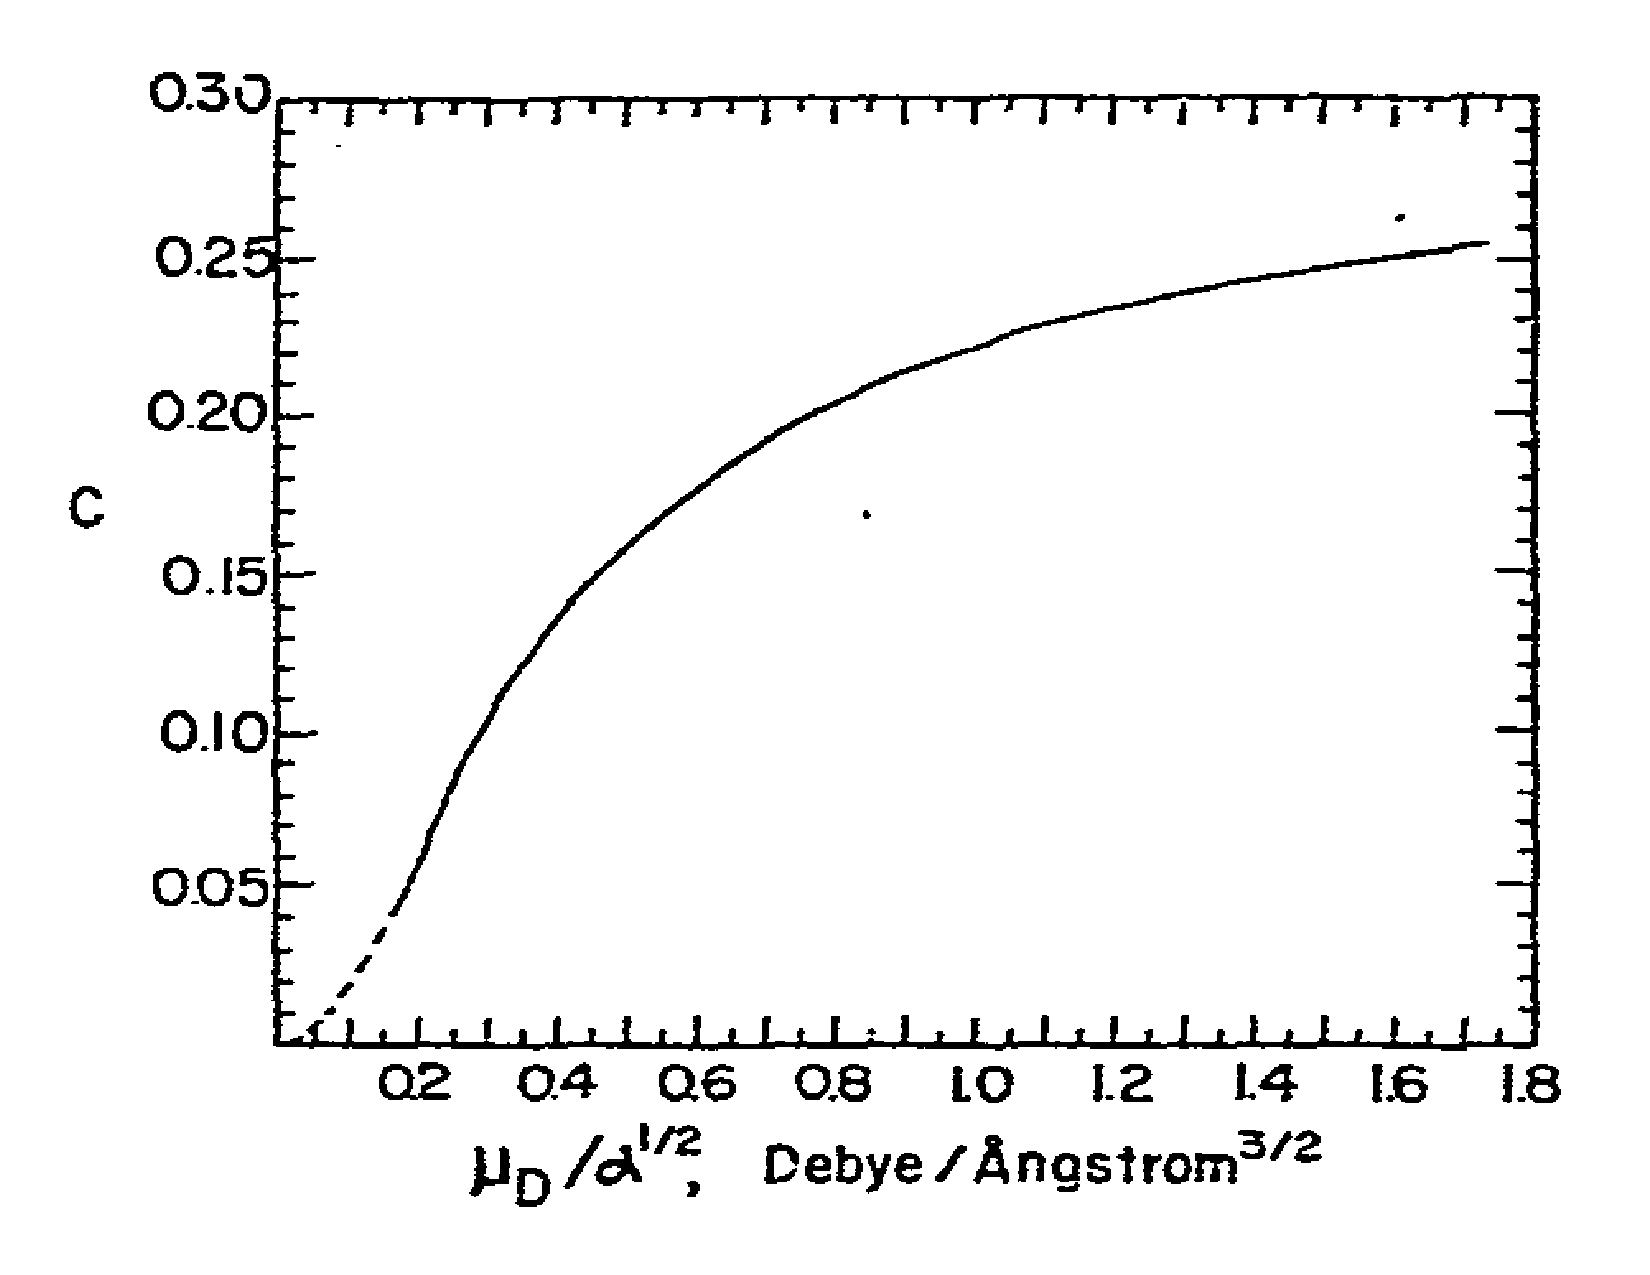
\includegraphics[width=0.8\textwidth]{images/ADO_C.pdf}
	\caption{Dipole locking constant $C$ parameterized by the dipole moment $\mu_D$ and polarizability $\alpha$.\cite{Su1973}}
\end{figure}
